\documentclass[11pt]{article}
\usepackage[notes]{la}
\lamodule{2}{3}{Characterizations of Invertible Matrices}
\laxdoc{1.4}
\laxdoc{1.9}
\laxdoc{2.1}
\laxdoc{2.2}

\begin{document}

\section{Characterizations of Invertible Matrices}

\begin{guide}
Chapter 1 taught us to ask many questions about a matrix. Do its columns span? Are they independent? Is the map one-to-one? Onto? Is there a pivot in every row? Does $A\bv{x}=\bv{0}$ have a nonzero solution? Section~2.2 added one more: can the map be undone? For a \emph{square} matrix these are not a dozen questions but a single question, asked in a dozen disguises. Why should that be true? And since any disguise will do, which one is the cheapest to check in a given problem?
\end{guide}

\textbf{By the end of this section you should be able to:}
\begin{itemize}
  \item explain why, for a square matrix, ``a pivot in every row'' and ``a pivot in every column'' say the same thing, and why this fails for rectangular matrices;
  \item state the Invertible Matrix Theorem, sort its twelve statements into four families (undo, pivots, uniqueness, existence), and follow its proof;
  \item decide whether a square matrix is invertible by choosing the cheapest suitable test, and name the statement of the theorem that you used;
  \item describe a singular matrix by exhibiting a witness for each failing statement;
  \item decide invertibility of a triangular matrix at a glance;
  \item explain why for square matrices $AB=I$ already implies $BA=I$, and why $AB$ is invertible only when $A$ and $B$ both are;
  \item decide when a linear transformation $\R^n\to\R^n$ is invertible, and write a formula for its inverse;
  \item recognise a nearly singular matrix and say why it is a problem in practice.
\end{itemize}

% ---------------------------------------------------------------------
\subsection*{Existence and uniqueness meet in a square matrix}

In Section~2.2 (Pause and think~\ref{2.2-think:whichundo}) we saw that a map can be undone only if two things happen. Every vector $\bv{y}$ must be an output (\emph{existence}: the map is onto), and each output must come from only one input (\emph{uniqueness}: the map is one-to-one). Chapter 1 translated both into pivots, and the two translations look different:
\begin{itemize}
  \item $A\bv{x}=\bv{b}$ has a solution for every $\bv{b}$ if and only if $A$ has a pivot in \textbf{every row} (Theorem~\ref{1.4-thm:existence}, Theorem~\ref{1.9-thm:ontoone});
  \item $A\bv{x}=\bv{0}$ has only the trivial solution, equivalently the map is one-to-one, if and only if $A$ has a pivot in \textbf{every column} (Theorem~\ref{1.9-thm:ontoone}).
\end{itemize}
For a general matrix these two conditions have nothing to do with each other.

\begin{exmp}{Three shapes}{shapes}
Let $P=\begin{bmatrix}1&0&0\\0&1&0\end{bmatrix}$, \ $Q=\begin{bmatrix}1&0\\0&1\\0&0\end{bmatrix}$ and $I_3$.

\textbf{$P$ is $2\times3$.} It has a pivot in both rows, so $P\bv{x}=\bv{b}$ is solvable for every $\bv{b}$ in $\R^2$ and the map $\R^3\to\R^2$ is onto. Column $3$ has no pivot, so $x_3$ is free and $P\bv{x}=\bv{0}$ has the nonzero solution $(0,0,1)$: the map is not one-to-one.

\textbf{$Q$ is $3\times2$.} It has a pivot in both columns, so $Q\bv{x}=\bv{0}$ has only the trivial solution and the map $\R^2\to\R^3$ is one-to-one. Row $3$ has no pivot, so $Q\bv{x}=(0,0,1)$ has no solution: the map is not onto.

\textbf{$I_3$ is $3\times3$.} Three pivots fill every row and every column at once: the map is both onto and one-to-one.
\end{exmp}

\begin{center}
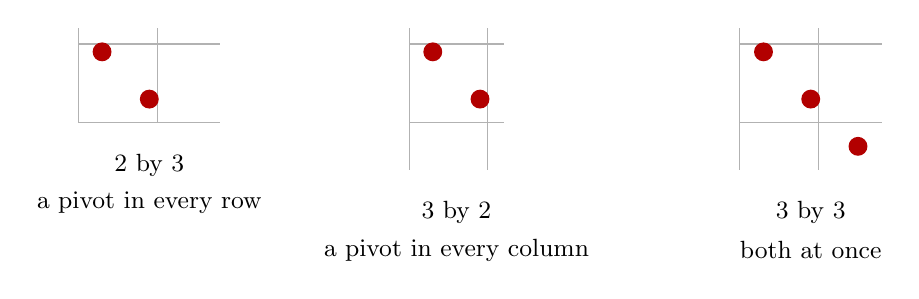
\begin{tikzpicture}[x=0.6cm,y=0.6cm]
  \draw[gray!60] (0,0) grid (3,2);
  \fill[red!70!black] (0.5,1.5) circle (0.2);
  \fill[red!70!black] (1.5,0.5) circle (0.2);
  \node at (1.5,-0.9) {\small 2 by 3};
  \node at (1.5,-1.7) {\small a pivot in every row};
  \begin{scope}[shift={(7,0)}]
    \draw[gray!60] (0,-1) grid (2,2);
    \fill[red!70!black] (0.5,1.5) circle (0.2);
    \fill[red!70!black] (1.5,0.5) circle (0.2);
    \node at (1,-1.9) {\small 3 by 2};
    \node at (1,-2.7) {\small a pivot in every column};
  \end{scope}
  \begin{scope}[shift={(14,0)}]
    \draw[gray!60] (0,-1) grid (3,2);
    \fill[red!70!black] (0.5,1.5) circle (0.2);
    \fill[red!70!black] (1.5,0.5) circle (0.2);
    \fill[red!70!black] (2.5,-0.5) circle (0.2);
    \node at (1.5,-1.9) {\small 3 by 3};
    \node at (1.5,-2.7) {\small both at once};
  \end{scope}
\end{tikzpicture}
\end{center}

\textbf{Figure.} Where the pivots sit. In the $2\times3$ grid a pivot reaches every row but only two of the three columns. In the $3\times2$ grid it is the other way round. Only in the square grid can the pivots fill the rows and the columns together.

What changes when the matrix is square? A pivot sits in exactly one row and in exactly one column, and no row or column holds two pivots. So the \emph{number} of pivots equals the number of rows that contain a pivot, and it also equals the number of columns that contain a pivot. If there are $n$ rows and $n$ columns, ``every row has a pivot'' and ``every column has a pivot'' both say ``there are $n$ pivots''.

\begin{thm}{The square pivot count}{squarecount}
Let $A$ be an $n\times n$ matrix. The following are equivalent:
\begin{enumerate}[label=(\alph*),itemsep=1pt]
  \item $A$ has a pivot in every row;
  \item $A$ has a pivot in every column;
  \item $A$ has $n$ pivot positions.
\end{enumerate}
\end{thm}

\begin{proof}
Each pivot position lies in one row and one column, and different pivots lie in different rows and in different columns. Hence the number of pivot positions equals the number of rows containing a pivot and equals the number of columns containing a pivot. A matrix with $n$ rows has a pivot in every row exactly when that number is $n$; the same is true for the $n$ columns.
\end{proof}

This small fact is the engine of the section: for square matrices \emph{existence is the same as uniqueness}.

\begin{kc}{Pivot bookkeeping}{pivotcount}
(a)~A $5\times5$ matrix has a pivot in every column. How many pivots does it have? Is $A\bv{x}=\bv{b}$ solvable for every $\bv{b}$? Can $A\bv{x}=\bv{0}$ have a nonzero solution? (b)~Repeat for a $5\times7$ matrix with a pivot in every row. (c)~Repeat for a $7\times5$ matrix with a pivot in every column.
\end{kc}

\begin{think}{Why exactly the square case?}{shapes}
(a)~Can a $2\times3$ matrix give a one-to-one map? Can a $3\times2$ matrix give an onto map? Use the figure. (b)~Existence and uniqueness are equivalent for $n\times n$ matrices, but are only \emph{unrelated} for other shapes. Describe in words which of the two a ``wide'' matrix (more columns than rows) can have, and which a ``tall'' matrix (more rows than columns) can have.
\end{think}

% ---------------------------------------------------------------------
\subsection*{The Invertible Matrix Theorem}

\begin{thm}{The Invertible Matrix Theorem}{imt}
Let $A$ be an $n\times n$ matrix. Then the following statements are equivalent: for a given $A$ they are either all true or all false.
\begin{enumerate}[label=(\alph*),itemsep=1pt]
  \item $A$ is an invertible matrix.
  \item $A$ is row equivalent to the identity matrix $I_n$.
  \item $A$ has $n$ pivot positions.
  \item The equation $A\bv{x}=\bv{0}$ has only the trivial solution.
  \item The columns of $A$ form a linearly independent set.
  \item The linear transformation $\bv{x}\mapsto A\bv{x}$ is one-to-one.
  \item The equation $A\bv{x}=\bv{b}$ has at least one solution for every $\bv{b}$ in $\R^n$.
  \item The columns of $A$ span $\R^n$.
  \item The linear transformation $\bv{x}\mapsto A\bv{x}$ maps $\R^n$ onto $\R^n$.
  \item There is an $n\times n$ matrix $C$ with $CA=I$.
  \item There is an $n\times n$ matrix $D$ with $AD=I$.
  \item $A\T$ is an invertible matrix.
\end{enumerate}
\end{thm}

The twelve statements fall into four families, and each family is one way of saying ``the map can be undone''.
\begin{itemize}
  \item \textbf{Undo:} (a), (j), (k), (l). There is an inverse, a left inverse, a right inverse, and the transpose has one too.
  \item \textbf{Pivots:} (b), (c). The row reduction ends in $I_n$ with $n$ pivots.
  \item \textbf{Uniqueness:} (d), (e), (f). Nothing is squashed: only $\bv{0}$ goes to $\bv{0}$, the columns are independent, no two inputs share an output.
  \item \textbf{Existence:} (g), (h), (i). Everything is reached: every $\bv{b}$ is an output, the columns span $\R^n$.
\end{itemize}

\begin{center}
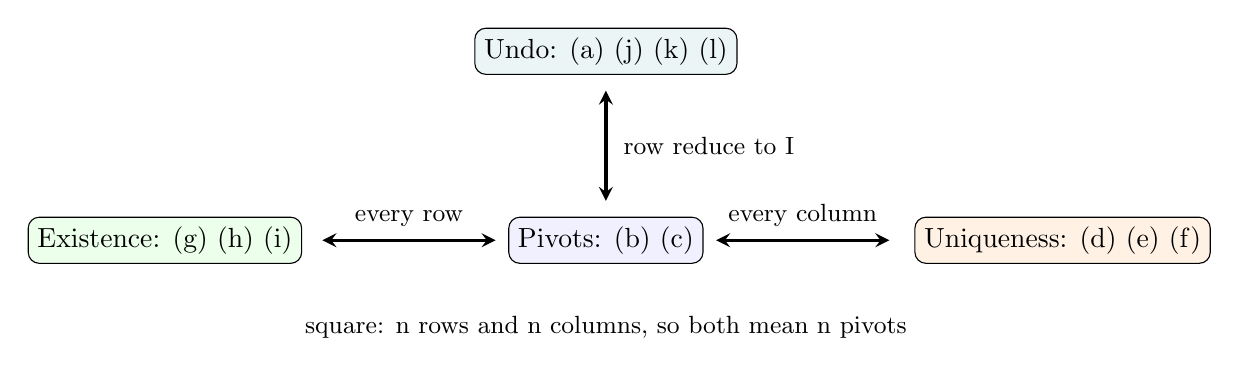
\begin{tikzpicture}[>=stealth,x=1cm,y=1cm]
  \node[draw,rounded corners,fill=teal!8] at (4,3.6) {Undo: (a) (j) (k) (l)};
  \node[draw,rounded corners,fill=blue!6] at (4,1.2) {Pivots: (b) (c)};
  \node[draw,rounded corners,fill=green!8] at (-1.6,1.2) {Existence: (g) (h) (i)};
  \node[draw,rounded corners,fill=orange!10] at (9.8,1.2) {Uniqueness: (d) (e) (f)};
  \draw[<->,very thick] (4,1.7)--(4,3.1);
  \node[right] at (4.1,2.4) {\small row reduce to I};
  \draw[<->,very thick] (0.4,1.2)--(2.6,1.2);
  \node[above] at (1.5,1.25) {\small every row};
  \draw[<->,very thick] (5.4,1.2)--(7.6,1.2);
  \node[above] at (6.5,1.25) {\small every column};
  \node at (4,0.1) {\small square: n rows and n columns, so both mean n pivots};
\end{tikzpicture}
\end{center}

\textbf{Figure.} The shape of the theorem. Chapter 1 gave the left and right families separately. Because the matrix is square, ``every row'' and ``every column'' both mean ``$n$ pivots'' (Theorem~\ref{thm:squarecount}), which links the two families through the middle; and the middle links to the inverse.

\begin{proof}
We prove the implications in a chain that touches every statement.

\emph{The circle} (a)$\Rightarrow$(j)$\Rightarrow$(d)$\Rightarrow$(c)$\Rightarrow$(b)$\Rightarrow$(a).

(a)$\Rightarrow$(j)~Take $C=A^{-1}$.

(j)$\Rightarrow$(d)~If $A\bv{x}=\bv{0}$, then $\bv{x}=I\bv{x}=(CA)\bv{x}=C(A\bv{x})=C\bv{0}=\bv{0}$.

(d)$\Rightarrow$(c)~Only the trivial solution means that there is no free variable, so every column has a pivot (Theorem~\ref{1.9-thm:ontoone}). Since $A$ is square, that is $n$ pivots (Theorem~\ref{thm:squarecount}).

(c)$\Rightarrow$(b)~There are $n$ pivots in $n$ rows and $n$ columns, one in each, and they step down and to the right, so they lie on the main diagonal. The reduced echelon form is $I_n$.

(b)$\Rightarrow$(a)~This is Theorem~\ref{2.2-thm:algorithm}.

\emph{The other statements.}

(a)$\Rightarrow$(k)~Take $D=A^{-1}$. (k)$\Rightarrow$(g)~For any $\bv{b}$, $A(D\bv{b})=(AD)\bv{b}=\bv{b}$, so $D\bv{b}$ is a solution. (g)$\Rightarrow$(c)~Solvability for every $\bv{b}$ gives a pivot in every row (Theorem~\ref{1.4-thm:existence}), which for a square matrix means $n$ pivots. So (k) and (g) are tied into the circle.

(g)$\Leftrightarrow$(h)$\Leftrightarrow$(i)~These are equivalent for \emph{every} matrix: Theorems~\ref{1.4-thm:existence} and~\ref{1.9-thm:ontoone}.

(d)$\Leftrightarrow$(e)$\Leftrightarrow$(f)~These are equivalent for every matrix: Section~1.7 and Theorem~\ref{1.9-thm:ontoone}.

(a)$\Leftrightarrow$(l)~If $A$ is invertible, so is $A\T$ (Theorem~\ref{2.2-thm:invprops}(c)). If $A\T$ is invertible, then applying the same theorem to $A\T$ shows that $(A\T)\T=A$ is invertible.
\end{proof}

Notice where the work is done. Almost every step only moves between descriptions of pivots. The \emph{only} step that produces an inverse out of nothing is (b)$\Rightarrow$(a), the algorithm of Section~2.2.

\begin{warn}[Square matrices only]
The theorem is about $n\times n$ matrices. For a $4\times3$ matrix whose columns are independent, statement (e) holds, but (g) and (h) are false (there are four rows and only three pivots), and ``invertible'' has no meaning. Never apply the theorem to a rectangular matrix, and never use it before checking that the matrix is square.
\end{warn}

\begin{exmp}{What follows from one fact}{consequences}
(i)~A $6\times6$ matrix $A$ has linearly independent columns. This is (e), so \emph{all} of the statements hold: $A$ is invertible, $A\bv{x}=\bv{b}$ has exactly one solution for every $\bv{b}$ in $\R^6$, the columns span $\R^6$, $A\T$ is invertible, so the \emph{rows} of $A$ are independent and span $\R^6$ too, and $A$ is row equivalent to $I_6$.

(ii)~A $5\times5$ matrix $B$ has a vector $\bv{b}$ for which $B\bv{x}=\bv{b}$ has no solution. This says that (g) is false, so every statement is false: $B$ is singular, $B\bv{x}=\bv{0}$ has a nonzero solution, the columns are dependent, $B$ has fewer than five pivots, the map is not one-to-one, and $B\T$ is also singular.

(iii)~A $4\times3$ matrix $C$ has independent columns. The theorem does not apply. We can still reason with pivots: three independent columns give three pivots, which cannot reach four rows. So $C\bv{x}=\bv{b}$ has a solution for \emph{some} $\bv{b}$ but not all, and when a solution exists it is unique.
\end{exmp}

\begin{kc}{Which statement is it?}{sort}
Each phrase describes one statement of the theorem. Give its letter. (i)~``There are no free variables.'' (ii)~``The map reaches every point of $\R^n$.'' (iii)~``The rows can be undone too.'' (iv)~``Reduced echelon form is $I_n$.'' (v)~``The system $A\bv{x}=\bv{b}$ never has more than one solution.''
\end{kc}

\begin{think}{Where is the inverse built?}{circle}
In the circle (a)$\Rightarrow$(j)$\Rightarrow$(d)$\Rightarrow$(c)$\Rightarrow$(b)$\Rightarrow$(a), which implications only reinterpret pivots and which one produces a matrix? Suppose someone claimed to have a proof that skipped (b)$\Rightarrow$(a). Why would it have to contain a different construction of an inverse somewhere?
\end{think}

% ---------------------------------------------------------------------
\subsection*{What a singular matrix looks like}

The theorem says that the twelve statements fail \emph{together}. So a singular matrix fails every one of them, and for each failing statement we can produce a concrete witness.

\begin{exmp}{Witnesses for a singular matrix}{witnesses}
Let $M=\begin{bmatrix}1&2&3\\0&1&1\\1&3&4\end{bmatrix}$. Row reduce:
\begin{align*}
\begin{bmatrix}1&2&3\\0&1&1\\1&3&4\end{bmatrix}
&\rops{R_3-R_1}
\begin{bmatrix}1&2&3\\0&1&1\\0&1&1\end{bmatrix}
\rops{R_3-R_2}
\begin{bmatrix}1&2&3\\0&1&1\\0&0&0\end{bmatrix}.
\end{align*}
There are two pivots, not three, so (c) fails and $M$ is singular. Every other statement fails as well, and we can say how:
\begin{itemize}
  \item (d), (f): column $3$ is free, and $M(1,1,-1)=\bv{0}$. So $M$ sends the nonzero vector $(1,1,-1)$ and the zero vector to the same output.
  \item (e): the columns satisfy $\bv{c}_1+\bv{c}_2-\bv{c}_3=\bv{0}$, a dependence relation with weights $(1,1,-1)$.
  \item (g), (i): reduce $[M\ \ \bv{e}_3]$:
  \begin{align*}
  \begin{amat}{ccc|c}1&2&3&0\\0&1&1&0\\1&3&4&1\end{amat}
  &\rops{R_3-R_1}
  \begin{amat}{ccc|c}1&2&3&0\\0&1&1&0\\0&1&1&1\end{amat}
  \rops{R_3-R_2}
  \begin{amat}{ccc|c}1&2&3&0\\0&1&1&0\\0&0&0&1\end{amat}.
  \end{align*}
  The last row says $0=1$, so $M\bv{x}=\bv{e}_3$ has no solution: $\bv{e}_3$ is not an output.
  \item (h): every column $(b_1,b_2,b_3)$ of $M$ satisfies $b_3=b_1+b_2$, so the columns span only that plane, not $\R^3$.
  \item (j): if $CM=I$ then $M(1,1,-1)=\bv{0}$ would give $(1,1,-1)=CM(1,1,-1)=\bv{0}$, which is false. So no left inverse exists.
  \item (k): if $MD=I$, the third column of $D$ would solve $M\bv{x}=\bv{e}_3$, which we just saw is impossible. So no right inverse exists.
  \item (l): row $1$ plus row $2$ minus row $3$ is $\bv{0}$, so $M\T(1,1,-1)=\bv{0}$ and $M\T$ is singular too.
\end{itemize}
\end{exmp}

\begin{think}{Negations}{negate}
(a)~Write the negation of (d), (g) and (j) in plain words, as properties of a singular matrix. (b)~To show that a matrix is \emph{not} invertible, why is one witness enough? (c)~In the example, the vector $(1,1,-1)$ appeared as the weights of a column dependence, as a null vector of $M$, and as a null vector of $M\T$. Are the first two the same fact? Is the third a coincidence of this particular matrix? Find a singular $2\times2$ matrix whose null vectors for $A$ and $A\T$ differ.
\end{think}

% ---------------------------------------------------------------------
\subsection*{Choosing the cheapest test}

The theorem is worth most when it lets us pick the statement that is easiest to check \emph{for the matrix in front of us}. Pivot counting always works, but it is not always the quickest.

\begin{proc}{Deciding whether a square matrix is invertible}{decide}
\begin{enumerate}
  \item \textbf{Look first.} Is the matrix $2\times2$? Triangular? A zero row or column? Two equal or proportional rows or columns? A permutation of the identity?
  \item \textbf{Use a shortcut if one applies:} $ad-bc$ for $2\times2$ (Theorem~\ref{2.2-thm:twobytwo}); nonzero diagonal for a triangular matrix (Theorem~\ref{thm:triangular}); a visible dependence among columns or among rows; the columns being the standard vectors in some order.
  \item \textbf{Otherwise row reduce $A$ itself} (not $[A\ \ I]$) to an echelon form and count pivots. Stop as soon as you know the answer: a zero row means singular, $n$ pivots means invertible.
  \item \textbf{Only if the inverse is needed} (or the solution for many right-hand sides), row reduce $[A\ \ I]$ as in Section~2.2.
\end{enumerate}
\end{proc}

\begin{exmp}{Six matrices, six quick tests}{sixtests}
Decide which matrices are invertible, using the cheapest test.

\textbf{(a)} $\begin{bmatrix}3&-6\\-1&2\end{bmatrix}$. A $2\times2$ matrix: $ad-bc=6-6=0$. Singular.

\textbf{(b)} $\begin{bmatrix}2&5&-1\\0&-3&4\\0&0&7\end{bmatrix}$. Upper triangular with diagonal entries $2,-3,7$, all nonzero: three pivots already in place. Invertible, with no row reduction at all.

\textbf{(c)} $\begin{bmatrix}1&4&1\\2&5&2\\3&6&3\end{bmatrix}$. Columns $1$ and $3$ are equal, so $\bv{c}_1-\bv{c}_3=\bv{0}$: dependent columns, statement (e) fails. Singular.

\textbf{(d)} $\begin{bmatrix}2&1&3\\4&2&6\\1&5&7\end{bmatrix}$. No two columns look proportional, but rows $1$ and $2$ are: $R_2=2R_1$. So the rows are dependent, hence $A\T$ has dependent columns and $A\T$ is singular, which by (l) means $A$ is singular.

\textbf{(e)} $\begin{bmatrix}1&0&0\\0&0&1\\0&1&0\end{bmatrix}$. The columns are $\bv{e}_1,\bv{e}_3,\bv{e}_2$: independent, so (e) holds. Invertible (it is its own inverse; compare the interchange matrices of Section~2.2).

\textbf{(f)} $\begin{bmatrix}1&2&3&4\\0&5&6&7\\0&0&0&8\\0&0&0&9\end{bmatrix}$. Upper triangular, but the third diagonal entry is $0$. Singular (Theorem~\ref{thm:triangular}; see also the repeated structure of rows $3$ and $4$).
\end{exmp}

\begin{exmp}{Count the pivots}{pivotex}
Is $A=\begin{bmatrix}1&2&-1\\2&5&0\\-3&-4&10\end{bmatrix}$ invertible?

\textbf{Solution.} No shortcut applies, so reduce $A$ to echelon form:
\begin{align*}
\begin{bmatrix}1&2&-1\\2&5&0\\-3&-4&10\end{bmatrix}
&\rops{R_2-2R_1,\ R_3+3R_1}
\begin{bmatrix}1&2&-1\\0&1&2\\0&2&7\end{bmatrix}
\rops{R_3-2R_2}
\begin{bmatrix}1&2&-1\\0&1&2\\0&0&3\end{bmatrix}.
\end{align*}
Three pivots: statement (c) holds, so $A$ is invertible. We did not need $[A\ \ I]$, and we do not know $A^{-1}$ yet. The theorem told us it exists, which is often all we need.
\end{exmp}

\begin{exmp}{A bigger matrix, and when to stop}{stopearly}
Is $B=\begin{bmatrix}1&2&0&1\\2&5&1&3\\1&3&1&3\\0&1&1&3\end{bmatrix}$ invertible?

\textbf{Solution.}
\begin{align*}
\begin{bmatrix}1&2&0&1\\2&5&1&3\\1&3&1&3\\0&1&1&3\end{bmatrix}
&\rops{R_2-2R_1,\ R_3-R_1}
\begin{bmatrix}1&2&0&1\\0&1&1&1\\0&1&1&2\\0&1&1&3\end{bmatrix}
\rops{R_3-R_2,\ R_4-R_2}
\begin{bmatrix}1&2&0&1\\0&1&1&1\\0&0&0&1\\0&0&0&2\end{bmatrix}\\[4pt]
&\rops{R_4-2R_3}
\begin{bmatrix}1&2&0&1\\0&1&1&1\\0&0&0&1\\0&0&0&0\end{bmatrix}.
\end{align*}
The pivots are in columns $1,2,4$: three pivots in a $4\times4$ matrix, so $B$ is singular. In fact we could have stopped one step earlier. The third column has no pivot, so $x_3$ is free; setting $x_3=1$ gives the nonzero solution $(2,-1,1,0)$ of $B\bv{x}=\bv{0}$. Check: the first row gives $2-2+0=0$, the second $4-5+1=0$, the third $2-3+1=0$, the fourth $0-1+1=0$.
\end{exmp}

\begin{exmp}{A parameter}{parameter}
For which values of $h$ is $C=\begin{bmatrix}1&2&h\\0&1&3\\2&5&7\end{bmatrix}$ invertible?

\textbf{Solution.} Row reduce, keeping $h$ in the formulas:
\begin{align*}
\begin{bmatrix}1&2&h\\0&1&3\\2&5&7\end{bmatrix}
&\rops{R_3-2R_1}
\begin{bmatrix}1&2&h\\0&1&3\\0&1&7-2h\end{bmatrix}
\rops{R_3-R_2}
\begin{bmatrix}1&2&h\\0&1&3\\0&0&4-2h\end{bmatrix}.
\end{align*}
The first two pivots are always there. A third pivot appears exactly when $4-2h\neq0$, that is, $h\neq2$. So $C$ is invertible for every $h\neq2$ and singular for $h=2$. At $h=2$ the third column is $(2,3,7)=-4\bv{c}_1+3\bv{c}_2$, so $C(-4,3,-1)=\bv{0}$.
\end{exmp}

\begin{kc}{Cheapest test}{cheapest}
Decide whether each matrix is invertible. Say which statement of the theorem (or which shortcut) you used. (a)~$\begin{bmatrix}2&4\\1&2\end{bmatrix}$; \ (b)~$\begin{bmatrix}1&0&2\\0&1&3\\0&0&0\end{bmatrix}$; \ (c)~$\begin{bmatrix}3&0&0&0\\1&-2&0&0\\5&4&6&0\\2&0&7&1\end{bmatrix}$; \ (d)~$\begin{bmatrix}0&0&1\\1&0&0\\0&1&0\end{bmatrix}$; \ (e)~$\begin{bmatrix}1&2&3\\4&5&6\\7&8&9\end{bmatrix}$.
\end{kc}

\begin{kc}{A parameter}{param}
For which $h$ is $D=\begin{bmatrix}1&0&h\\0&1&2\\1&1&3\end{bmatrix}$ singular? For that $h$ find a nonzero $\bv{x}$ with $D\bv{x}=\bv{0}$.
\end{kc}

\begin{think}{Which test would you trust?}{cheapest}
(a)~A $50\times50$ matrix arrives as a spreadsheet of decimal numbers. Which statement of the theorem would you test, and why not (g) or (f)? Notice that (g) and (f) quantify over \emph{infinitely many} vectors, while (c) needs only a finite computation. (b)~If $A$ is a product of matrices that you already know to be invertible, which fact makes the test unnecessary? (c)~For which kinds of matrices is the $2\times2$ formula of Section~2.2 useless, and for which kinds is full row reduction wasteful?
\end{think}

% ---------------------------------------------------------------------
\subsection*{Triangular matrices}

A matrix is \emph{upper triangular} if all entries below the diagonal are $0$ and \emph{lower triangular} if all entries above it are $0$.

\begin{thm}{Triangular matrices}{triangular}
A triangular $n\times n$ matrix is invertible if and only if every diagonal entry is nonzero.
\end{thm}

\begin{proof}
First let $A$ be upper triangular. If all diagonal entries are nonzero, $A$ is already in echelon form with a pivot in each of the $n$ diagonal positions, so (c) holds and $A$ is invertible.

Now suppose some diagonal entry is $0$ and let $k$ be the first one, $a_{kk}=0$. Each of the first $k$ columns has all its entries below the diagonal equal to $0$, and column $k$ has $a_{kk}=0$ as well. So the first $k$ columns have nonzero entries only in rows $1,\dots,k-1$: they are $k$ vectors with only $k-1$ possibly nonzero entries (if $k=1$, the first column is the zero vector). By Section~1.7 more vectors than entries are linearly dependent, so (e) fails and $A$ is singular.

If $A$ is lower triangular, then $A\T$ is upper triangular with the same diagonal, and $A$ is invertible exactly when $A\T$ is (statement (l)).
\end{proof}

\begin{kc}{Triangular}{triangular}
Which of these are invertible? \ (a)~$\begin{bmatrix}2&7&1\\0&-1&5\\0&0&3\end{bmatrix}$; \ (b)~$\begin{bmatrix}4&0&0\\1&0&0\\2&3&5\end{bmatrix}$; \ (c)~$\begin{bmatrix}1&2&3&4\\0&1&2&3\\0&0&1&2\\0&0&0&0\end{bmatrix}$. For each singular one, find a nonzero $\bv{x}$ with $A\bv{x}=\bv{0}$ or $A\T\bv{x}=\bv{0}$.
\end{kc}

% ---------------------------------------------------------------------
\subsection*{One-sided inverses and products}

The definition of an inverse asks for two equations, $CA=I$ and $AC=I$ (Definition~\ref{2.2-def:inverse}). The theorem says that for square matrices one of them is enough: (j) and (k) are each equivalent to (a).

\begin{thm}{One product is enough}{onesided}
Let $A$ and $B$ be $n\times n$ matrices. If $AB=I$, then $BA=I$ as well. Hence $A$ and $B$ are both invertible, $B=A^{-1}$ and $A=B^{-1}$.
\end{thm}

\begin{proof}
$AB=I$ says that $B$ is a right inverse of $A$, statement (k). By the theorem $A$ is invertible. Then $B=(A^{-1}A)B=A^{-1}(AB)=A^{-1}$, and so $BA=A^{-1}A=I$.
\end{proof}

\begin{exmp}{Check only one product}{oneproduct}
Let $A=\begin{bmatrix}1&1&1\\0&1&1\\0&0&1\end{bmatrix}$ and $B=\begin{bmatrix}1&-1&0\\0&1&-1\\0&0&1\end{bmatrix}$. Then
\[
AB=\begin{bmatrix}1&1&1\\0&1&1\\0&0&1\end{bmatrix}\begin{bmatrix}1&-1&0\\0&1&-1\\0&0&1\end{bmatrix}=\begin{bmatrix}1&0&0\\0&1&0\\0&0&1\end{bmatrix}.
\]
That is all we need: $A$ is invertible with $A^{-1}=B$. The other product is automatically
\[
BA=\begin{bmatrix}1&-1&0\\0&1&-1\\0&0&1\end{bmatrix}\begin{bmatrix}1&1&1\\0&1&1\\0&0&1\end{bmatrix}=\begin{bmatrix}1&0&0\\0&1&0\\0&0&1\end{bmatrix},
\]
which we computed only to see the theorem at work. By hand, one $3\times3$ product instead of two is a real saving.
\end{exmp}

\begin{warn}[Rectangular matrices break this]
The statement fails for non-square matrices. Let $A=\begin{bmatrix}1&0&0\\0&1&0\end{bmatrix}$ ($2\times3$) and $B=\begin{bmatrix}1&0\\0&1\\0&0\end{bmatrix}$ ($3\times2$). Then $AB=I_2$, but $BA=\begin{bmatrix}1&0&0\\0&1&0\\0&0&0\end{bmatrix}\neq I_3$. Neither matrix is invertible: the square case is special.
\end{warn}

\begin{exmp}{An inverse from an equation}{fibonacci}
The matrix $A=\begin{bmatrix}1&1\\1&0\end{bmatrix}$ satisfies
\[
A^2=\begin{bmatrix}1&1\\1&0\end{bmatrix}\begin{bmatrix}1&1\\1&0\end{bmatrix}=\begin{bmatrix}2&1\\1&1\end{bmatrix},\qquad A^2-A=\begin{bmatrix}1&0\\0&1\end{bmatrix}=I.
\]
Factor the left side: $A(A-I)=I$. By Theorem~\ref{thm:onesided} $A$ is invertible, and $A^{-1}=A-I=\begin{bmatrix}0&1\\1&-1\end{bmatrix}$. Check with the $2\times2$ formula: $ad-bc=0-1=-1$ and $\frac1{-1}\begin{bmatrix}0&-1\\-1&1\end{bmatrix}=\begin{bmatrix}0&1\\1&-1\end{bmatrix}$. The same trick works for any square $A$ that satisfies an equation of the form $A^2+pA+qI=\mathbf{0}$ with $q\neq0$: then $A(A+pI)=-qI$.
\end{exmp}

\begin{thm}{Invertible products}{products}
Let $A$ and $B$ be $n\times n$ matrices. Then $AB$ is invertible if and only if both $A$ and $B$ are invertible.
\end{thm}

\begin{proof}
($\Leftarrow$)~This is Theorem~\ref{2.2-thm:invprops}(b).

($\Rightarrow$)~Let $C=(AB)^{-1}$. Then $A(BC)=(AB)C=I$, so $A$ has a right inverse, statement (k), and is invertible. Also $(CA)B=C(AB)=I$, so $B$ has a left inverse, statement (j), and is invertible.
\end{proof}

Equivalently, if $A$ or $B$ is singular, then so are $AB$ \emph{and} $BA$. This is the reason why a product of matrices can never repair a squashed direction.

\begin{kc}{One product}{onesided}
Let $B=\begin{bmatrix}2&1\\5&3\end{bmatrix}$ and $C=\begin{bmatrix}3&-1\\-5&2\end{bmatrix}$. (a)~Compute $BC$. (b)~Without computing $CB$, what is it and why? (c)~What is $B^{-1}$?
\end{kc}

\begin{kc}{Singular products}{singprod}
$A$ and $B$ are $n\times n$ and $AB$ is singular. Which of these can be concluded? (a)~$A$ is singular; (b)~$B$ is singular; (c)~at least one of $A$, $B$ is singular. Give examples where (a) or (b) fails.
\end{kc}

\begin{think}{Left or right?}{leftright}
(a)~Let $A$ be $2\times3$. Can there be a $3\times2$ matrix $C$ with $CA=I_3$? (Think about $A\bv{x}=\bv{0}$.) (b)~Give a $3\times2$ matrix $A$ and a $2\times3$ matrix $C$ with $CA=I_2$. Is $AC=I_3$? (c)~How does the theorem rescue us when $A$ is square?
\end{think}

\begin{think}{Finite and infinite}{finite}
For a function $f$ from a \emph{finite} set to itself, ``one-to-one'' and ``onto'' are equivalent: if no two elements share an output, the outputs fill up the whole set, and conversely. For the function $f(n)=n+1$ on the infinite set $\{1,2,3,\dots\}$, this fails: it is one-to-one but $1$ is never an output. (a)~Where in the proof of the Invertible Matrix Theorem did ``finiteness'' enter? (b)~Is this a hint that the theorem cannot extend to infinite lists of vectors?
\end{think}

% ---------------------------------------------------------------------
\subsection*{Invertible linear transformations}

Matrix multiplication is composition (Theorem~\ref{2.1-thm:composite}), so undoing a matrix is undoing a linear transformation.

\begin{defn}{Invertible transformation}{invtrans}
A linear transformation $T:\R^n\to\R^n$ is \emph{invertible} if there is a function $S:\R^n\to\R^n$ with
\[
S(T(\bv{x}))=\bv{x}\quad\text{and}\quad T(S(\bv{y}))=\bv{y}\qquad\text{for all }\bv{x},\bv{y}\text{ in }\R^n.
\]
\end{defn}

\begin{thm}{Invertible transformations}{invtrans}
Let $T:\R^n\to\R^n$ be linear with standard matrix $A$ (Definition~\ref{1.9-def:stdmat}). Then $T$ is invertible if and only if $A$ is invertible. In that case the function $S$ is unique and is the linear transformation $S(\bv{y})=A^{-1}\bv{y}$. We write $S=T^{-1}$.
\end{thm}

\begin{proof}
Suppose $T$ is invertible. For every $\bv{y}$ the equation $T(\bv{x})=\bv{y}$ has the solution $\bv{x}=S(\bv{y})$, so $T$ is onto, which is statement (i), and $A$ is invertible.

Conversely, let $A$ be invertible and put $S(\bv{y})=A^{-1}\bv{y}$. Then $S(T(\bv{x}))=A^{-1}A\bv{x}=\bv{x}$ and $T(S(\bv{y}))=AA^{-1}\bv{y}=\bv{y}$, so $T$ is invertible.

For uniqueness, suppose $S'$ is any function with $S'(T(\bv{x}))=\bv{x}$ for all $\bv{x}$. For every $\bv{y}$ we have $\bv{y}=T(S(\bv{y}))$, hence $S'(\bv{y})=S'(T(S(\bv{y})))=S(\bv{y})$.
\end{proof}

\begin{exmp}{The formula for $T^{-1}$}{tinverse}
Let $T(x_1,x_2,x_3)=(x_1+x_2,\ x_2+x_3,\ x_3)$. Its standard matrix is $A=\begin{bmatrix}1&1&0\\0&1&1\\0&0&1\end{bmatrix}$, upper triangular with diagonal entries $1$, so $T$ is invertible by Theorem~\ref{thm:triangular}. To find $T^{-1}$, solve $T(\bv{x})=\bv{y}$ from the bottom up: $x_3=y_3$, \ $x_2=y_2-x_3=y_2-y_3$, \ $x_1=y_1-x_2=y_1-y_2+y_3$. So
\[
T^{-1}(y_1,y_2,y_3)=(y_1-y_2+y_3,\ y_2-y_3,\ y_3),\qquad A^{-1}=\begin{bmatrix}1&-1&1\\0&1&-1\\0&0&1\end{bmatrix}.
\]
Check with $\bv{x}=(1,2,3)$: $T(\bv{x})=(3,5,3)$ and $T^{-1}(3,5,3)=(3-5+3,\ 5-3,\ 3)=(1,2,3)$. \ $\checkmark$
\end{exmp}

\begin{exmp}{A transformation that cannot be undone}{notinvt}
Let $T(x_1,x_2,x_3)=(x_1-x_2,\ x_2-x_3,\ x_3-x_1)$, with standard matrix $A=\begin{bmatrix}1&-1&0\\0&1&-1\\-1&0&1\end{bmatrix}$. The three outputs always add up to $0$: $(x_1-x_2)+(x_2-x_3)+(x_3-x_1)=0$. So $T$ misses every vector whose entries do not add to $0$, such as $(1,0,0)$, and is not onto. Equivalently $T(1,1,1)=\bv{0}$, so $T$ is not one-to-one. By Theorem~\ref{thm:invtrans}, $T$ is not invertible; the columns of $A$ add to $\bv{0}$, so $A$ is singular.
\end{exmp}

\begin{kc}{Undo these maps}{tinverse}
(a)~$T(x_1,x_2)=(x_1+2x_2,\ 3x_1+7x_2)$: show that $T$ is invertible and find $T^{-1}$. (b)~$U(x_1,x_2)=(x_1-2x_2,\ -3x_1+6x_2)$: is $U$ invertible? Find a nonzero vector that $U$ sends to $\bv{0}$.
\end{kc}

\begin{think}{Onto is enough}{ontoinv}
Let $T$ and $U$ be linear transformations from $\R^n$ to $\R^n$ with $T(U(\bv{x}))=\bv{x}$ for all $\bv{x}$. Is it true that $U(T(\bv{x}))=\bv{x}$ for all $\bv{x}$? Translate into matrices and use Theorem~\ref{thm:onesided}.
\end{think}

% ---------------------------------------------------------------------
\subsection*{A caution from practice: nearly singular matrices}

In exact arithmetic a matrix is either singular or not. Computers round numbers, and a matrix can be invertible but so close to singular that tiny errors matter.

\begin{exmp}{A tiny change, a large effect}{nearly}
Let $A=\begin{bmatrix}1&1\\1&1.0001\end{bmatrix}$. Then $ad-bc=1.0001-1=0.0001\neq0$, so $A$ is invertible, with
\[
A^{-1}=\frac1{0.0001}\begin{bmatrix}1.0001&-1\\-1&1\end{bmatrix}=\begin{bmatrix}10001&-10000\\-10000&10000\end{bmatrix}.
\]
The system $A\bv{x}=(2,\ 2.0001)$ has the solution $\bv{x}=(1,1)$. Change the second right-hand entry by $0.0001$, to $2.0002$ (about $0.005\%$ of the data):
\[
A^{-1}\begin{bmatrix}2\\2.0002\end{bmatrix}=\begin{bmatrix}10001\cdot2-10000\cdot2.0002\\-10000\cdot2+10000\cdot2.0002\end{bmatrix}=\begin{bmatrix}20002-20002\\2\end{bmatrix}=\begin{bmatrix}0\\2\end{bmatrix}.
\]
The solution moves from $(1,1)$ to $(0,2)$: it changes by as much as its own size.
\end{exmp}

\begin{center}
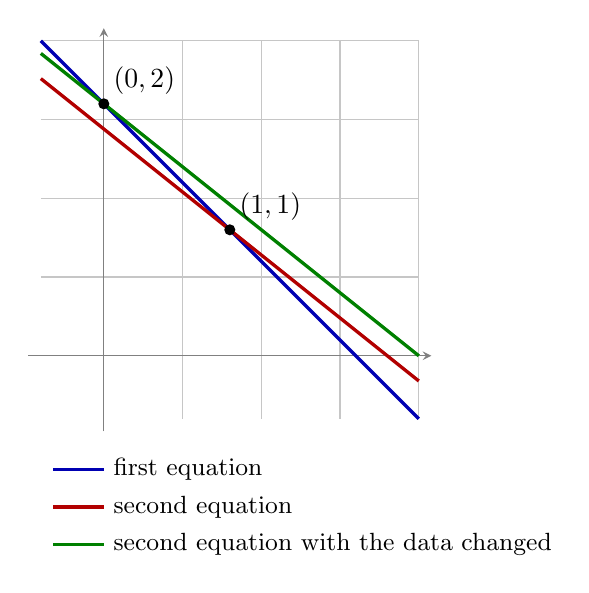
\begin{tikzpicture}[x=1.6cm,y=1.6cm,>=stealth]
  \draw[gray!45] (-0.5,-0.5) grid (2.5,2.5);
  \draw[->,gray] (-0.6,0)--(2.6,0); \draw[->,gray] (0,-0.6)--(0,2.6);
  \draw[very thick,blue!70!black] (-0.5,2.5)--(2.5,-0.5);
  \draw[very thick,red!70!black] (-0.5,2.2)--(2.5,-0.2);
  \draw[very thick,green!50!black] (-0.5,2.4)--(2.5,0);
  \fill (1,1) circle (2pt);
  \fill (0,2) circle (2pt);
  \node[above right] at (1,1) {$(1,1)$};
  \node[above right] at (0,2) {$(0,2)$};
  \draw[very thick,blue!70!black] (-0.4,-0.9)--(0,-0.9);
  \node[right] at (0,-0.9) {\small first equation};
  \draw[very thick,red!70!black] (-0.4,-1.2)--(0,-1.2);
  \node[right] at (0,-1.2) {\small second equation};
  \draw[very thick,green!50!black] (-0.4,-1.5)--(0,-1.5);
  \node[right] at (0,-1.5) {\small second equation with the data changed};
\end{tikzpicture}
\end{center}

\textbf{Figure.} Two nearly parallel lines. The first equation $x_1+x_2=2$ is crossed by the second equation at $(1,1)$; when the data of the second equation is changed only slightly, the crossing slides along the first line to $(0,2)$. (The angle between the lines is exaggerated; for the matrix above the two lines are almost indistinguishable on a drawing.) A matrix whose columns are almost dependent has a huge inverse (here $10^4$), and errors in the data are multiplied by it.

\begin{think}{Singular or nearly singular?}{sensitivity}
(a)~In the example, by what percentage did the data change and by what percentage did the solution change? (b)~How does the size of the entries of $A^{-1}$ explain this? (c)~A computer that keeps only four significant digits rounds $1.0001$ to $1.000$. Which matrix does it see? What does the theorem say about that matrix?
\end{think}

\begin{think}{Explain it to a classmate}{explain}
Let $A$ be a square matrix for which $A\bv{x}=\bv{0}$ has only the trivial solution. In your own words, with a sketch if you like, explain why $A\bv{x}=\bv{b}$ must then be solvable for every $\bv{b}$. Then explain why the same argument fails for a $5\times3$ matrix.
\end{think}

\subsection*{Summary}
\begin{itemize}
  \item For a square matrix, a pivot in every row, a pivot in every column and $n$ pivots are the same condition (Theorem~\ref{thm:squarecount}): \textbf{existence and uniqueness coincide}. For rectangular matrices they are unrelated.
  \item \textbf{Invertible Matrix Theorem.} For an $n\times n$ matrix the following are equivalent: invertible; row equivalent to $I_n$; $n$ pivots; $A\bv{x}=\bv{0}$ only trivial; columns independent; map one-to-one; $A\bv{x}=\bv{b}$ solvable for every $\bv{b}$; columns span $\R^n$; map onto; left inverse; right inverse; $A\T$ invertible. Four families: undo, pivots, uniqueness, existence. The theorem is only for square matrices.
  \item A singular matrix fails all twelve at once, and each failing statement has a concrete witness.
  \item \textbf{Cheapest test.} $2\times2$: $ad-bc$. Triangular: nonzero diagonal. Visible dependence among rows or columns: singular. Otherwise row reduce $A$ and count pivots. Compute $A^{-1}$ only when it is needed.
  \item For square matrices one product suffices: $AB=I\Rightarrow BA=I$. And $AB$ is invertible if and only if $A$ and $B$ both are.
  \item A linear transformation $T:\R^n\to\R^n$ is invertible exactly when its standard matrix is, and then $T^{-1}(\bv{y})=A^{-1}\bv{y}$.
  \item A matrix can be invertible and still so close to singular that small errors in the data are hugely amplified.
\end{itemize}

\subsection*{Questions to think about before the next section}
\begin{enumerate}
  \item For $2\times2$ matrices the number $ad-bc$ decides invertibility. The theorem does not give a formula like that for $3\times3$ matrices. Is there one number, computed from the nine entries, that is zero exactly when $A$ is singular? What should it measure in $\R^3$?
  \item Let $A=\begin{bmatrix}2&0\\0&3\end{bmatrix}$. For which numbers $\lambda$ is $A-\lambda I$ singular? What does a nonzero solution of $(A-\lambda I)\bv{x}=\bv{0}$ say about $A\bv{x}$?
  \item The columns of an invertible $n\times n$ matrix are independent and span $\R^n$. Does \emph{every} point of $\R^n$ then have a unique description as a combination of those columns? What would you call such a set of columns?
\end{enumerate}

\subsection*{Answers and discussion}
\begin{description}[leftmargin=0pt,itemsep=5pt]
  \item[Knowledge Check \ref{kc:pivotcount}.] (a)~Five pivots (one per column). With five rows they fill every row, so $A\bv{x}=\bv{b}$ is solvable for every $\bv{b}$, and $A\bv{x}=\bv{0}$ has only the trivial solution. (b)~Five pivots, one in each of the five rows, so $A\bv{x}=\bv{b}$ is solvable for every $\bv{b}$; but only five of the seven columns have a pivot, so there are two free variables and $A\bv{x}=\bv{0}$ has nonzero solutions. (c)~Five pivots in five columns, so $A\bv{x}=\bv{0}$ has only the trivial solution; but there are seven rows, so two rows have no pivot and $A\bv{x}=\bv{b}$ is not solvable for every $\bv{b}$.
  \item[Knowledge Check \ref{kc:sort}.] (i)~(d) (equivalently (e) or (f); also (c)). (ii)~(i) (equivalently (g) or (h)). (iii)~(l). (iv)~(b). (v)~(f), which is the same as (d): two different solutions $\bv{x},\bv{x}'$ of $A\bv{x}=\bv{b}$ would give the nonzero solution $\bv{x}-\bv{x}'$ of $A\bv{x}=\bv{0}$.
  \item[Knowledge Check \ref{kc:cheapest}.] (a)~$ad-bc=4-4=0$: singular. (b)~A zero row, so at most two pivots (statement (c) fails): singular. (c)~Lower triangular with diagonal entries $3,-2,6,1$, all nonzero: invertible (Theorem~\ref{thm:triangular}). (d)~The columns are $\bv{e}_2,\bv{e}_3,\bv{e}_1$: independent, so invertible (statement (e)). (e)~No shortcut: reduce.
  \begin{align*}
  \begin{bmatrix}1&2&3\\4&5&6\\7&8&9\end{bmatrix}
  &\rops{R_2-4R_1,\ R_3-7R_1}
  \begin{bmatrix}1&2&3\\0&-3&-6\\0&-6&-12\end{bmatrix}
  \rops{R_3-2R_2}
  \begin{bmatrix}1&2&3\\0&-3&-6\\0&0&0\end{bmatrix}.
  \end{align*}
  Two pivots: singular. Indeed $\bv{c}_1-2\bv{c}_2+\bv{c}_3=\bv{0}$.
  \item[Knowledge Check \ref{kc:param}.]
  \begin{align*}
  \begin{bmatrix}1&0&h\\0&1&2\\1&1&3\end{bmatrix}
  &\rops{R_3-R_1}
  \begin{bmatrix}1&0&h\\0&1&2\\0&1&3-h\end{bmatrix}
  \rops{R_3-R_2}
  \begin{bmatrix}1&0&h\\0&1&2\\0&0&1-h\end{bmatrix}.
  \end{align*}
  The third pivot is missing exactly when $h=1$, so $D$ is singular only for $h=1$. Then $x_3$ is free and $x_2=-2x_3$, $x_1=-x_3$: take $\bv{x}=(-1,-2,1)$. Check: $-1+0+1=0$, \ $-2+2=0$, \ $-1-2+3=0$.
  \item[Knowledge Check \ref{kc:triangular}.] (a)~Upper triangular with diagonal $2,-1,3$: invertible. (b)~Lower triangular with $a_{22}=0$: singular. Columns $2$ and $3$ are $(0,0,3)$ and $(0,0,5)$, so $5\bv{c}_2-3\bv{c}_3=\bv{0}$, that is, $A(0,5,-3)=\bv{0}$. (c)~Upper triangular with $a_{44}=0$: singular. The fourth row is zero, so $A\T(0,0,0,1)=\bv{0}$. Also $A(0,1,-2,1)=\bv{0}$: the rows give $0+2-6+4$, \ $1-4+3$, \ $-2+2$, and $0$.
  \item[Knowledge Check \ref{kc:onesided}.] (a)~$BC=\begin{bmatrix}6-5&-2+2\\15-15&-5+6\end{bmatrix}=\begin{bmatrix}1&0\\0&1\end{bmatrix}$. (b)~$CB=I$ too: both matrices are $2\times2$, and by Theorem~\ref{thm:onesided} one product equal to $I$ forces the other. (Direct check: $\begin{bmatrix}6-5&3-3\\-10+10&-5+6\end{bmatrix}=I$.) (c)~$B^{-1}=C$.
  \item[Knowledge Check \ref{kc:singprod}.] Only (c). The theorem says $AB$ is invertible exactly when both are, so if $AB$ is singular, at least one factor is. But (a) can fail: $A=I$ and $B=\begin{bmatrix}1&0\\0&0\end{bmatrix}$ give $AB=B$ singular while $A$ is invertible. And (b) can fail: $A=\begin{bmatrix}1&0\\0&0\end{bmatrix}$ and $B=I$.
  \item[Knowledge Check \ref{kc:tinverse}.] (a)~The standard matrix is $\begin{bmatrix}1&2\\3&7\end{bmatrix}$ with $ad-bc=7-6=1\neq0$, so $T$ is invertible, with matrix $\begin{bmatrix}7&-2\\-3&1\end{bmatrix}$, so $T^{-1}(y_1,y_2)=(7y_1-2y_2,\ -3y_1+y_2)$. Check: $T(1,1)=(3,10)$ and $T^{-1}(3,10)=(21-20,\ -9+10)=(1,1)$. (b)~The standard matrix is $\begin{bmatrix}1&-2\\-3&6\end{bmatrix}$ with $ad-bc=6-6=0$, so $U$ is not invertible. $U(2,1)=(2-2,\ -6+6)=(0,0)$. The outputs are all of the form $(u,-3u)$, a line, so $U$ is neither one-to-one nor onto.
  \item[Pause and think \ref{think:shapes}.] (a)~A $2\times3$ matrix has at most $2$ pivots but $3$ columns, so some column is free and the map is not one-to-one. A $3\times2$ matrix has at most $2$ pivots but $3$ rows, so some row has no pivot and the map is not onto. (b)~A wide matrix can be onto but never one-to-one (more unknowns than equations: free variables). A tall matrix can be one-to-one but never onto (more equations than unknowns: some right-hand side is inconsistent). Only for the square shape can the same pivots serve both purposes.
  \item[Pause and think \ref{think:circle}.] The steps (a)$\Rightarrow$(j) (take $C=A^{-1}$), (j)$\Rightarrow$(d), (d)$\Rightarrow$(c) and (c)$\Rightarrow$(b) only rewrite statements or count pivots. The step (b)$\Rightarrow$(a) is the one that produces a matrix: the product of elementary matrices $E_p\cdots E_1$ that carries $A$ to $I$. Any other proof must build an inverse somewhere too, for example by solving $A\bv{x}=\bv{e}_j$ for each $j$ and using the solutions as the columns of a matrix $D$ with $AD=I$. Without such a construction, statements about pivots could never produce a matrix with the two properties of an inverse.
  \item[Pause and think \ref{think:negate}.] (a)~Not (d): $A\bv{x}=\bv{0}$ has a nonzero solution. Not (g): there is a $\bv{b}$ for which $A\bv{x}=\bv{b}$ has no solution. Not (j): no matrix $C$ satisfies $CA=I$. (b)~If $A$ were invertible, all twelve statements would be true. A single false statement therefore rules out invertibility. (c)~The first two are the same fact, because $A\bv{x}=x_1\bv{c}_1+\cdots+x_n\bv{c}_n$: a null vector is exactly a vector of weights of a dependence relation. The third is a coincidence of $M$ (here the dependence relation among the rows has the same weights as the one among the columns). In general they differ: for $A=\begin{bmatrix}1&2\\3&6\end{bmatrix}$ we have $A(2,-1)=\bv{0}$ but $A\T(2,-1)=(-1,-2)\neq\bv{0}$; instead $A\T(3,-1)=\bv{0}$.
  \item[Pause and think \ref{think:cheapest}.] (a)~Test (c): row reduce and count pivots, a finite computation (a few thousand arithmetic steps). Statements (g) and (f) quantify over all vectors $\bv{b}$ or all pairs $\bv{x},\bv{x}'$, which cannot be tested one by one. (b)~Theorem~\ref{2.2-thm:invprops}(b) or Theorem~\ref{thm:products}: a product of invertible matrices is invertible. (c)~The $2\times2$ formula is useless for $n\ge3$; row reduction is wasteful for $2\times2$, triangular matrices, permutation matrices and matrices with visibly dependent rows or columns, where one glance decides.
  \item[Pause and think \ref{think:leftright}.] (a)~No. A $2\times3$ matrix $A$ has a free variable, so $A\bv{x}=\bv{0}$ has a nonzero solution, and then $CA\bv{x}=\bv{0}\neq\bv{x}$, so $CA\neq I_3$. (b)~$A=\begin{bmatrix}1&0\\0&1\\0&0\end{bmatrix}$ and $C=\begin{bmatrix}1&0&0\\0&1&0\end{bmatrix}$ give $CA=I_2$, but $AC=\begin{bmatrix}1&0&0\\0&1&0\\0&0&0\end{bmatrix}\neq I_3$. (c)~For square $A$, $CA=I$ is statement (j), so all twelve statements hold, in particular $A$ is invertible and $C=A^{-1}$ satisfies $AC=I$.
  \item[Pause and think \ref{think:finite}.] (a)~In Theorem~\ref{thm:squarecount}: a square matrix has the same \emph{finite} number $n$ of rows and columns, and the pivots are counted once by rows and once by columns. (b)~Yes: for infinite lists the analogue of the theorem is false. The ``shift'' $(x_1,x_2,x_3,\dots)\mapsto(0,x_1,x_2,\dots)$ is a linear map that is one-to-one but not onto, and it has a left inverse (shift back) but no right inverse. The theorem uses in an essential way that $\R^n$ is finite dimensional.
  \item[Pause and think \ref{think:ontoinv}.] Yes. Let $A$ and $B$ be the standard matrices of $T$ and $U$. The standard matrix of $T\circ U$ is $AB$ (Theorem~\ref{2.1-thm:composite}), and $T(U(\bv{x}))=\bv{x}$ for all $\bv{x}$ means $AB\bv{x}=\bv{x}$ for all $\bv{x}$, so $AB=I$. By Theorem~\ref{thm:onesided}, $BA=I$, that is, $U(T(\bv{x}))=\bv{x}$ for all $\bv{x}$.
  \item[Pause and think \ref{think:sensitivity}.] (a)~The data changed by $0.0001$ in one entry of $(2,\ 2.0001)$, which has length about $2.83$: roughly $0.0035\%$ (or $0.005\%$ of the entry). The solution moved from $(1,1)$ to $(0,2)$, by $(-1,1)$, whose length $\sqrt2$ equals the length of $(1,1)$: a $100\%$ change. (b)~The entries of $A^{-1}$ are of size $10^4$. An error $\Delta\bv{b}$ in the data produces the error $A^{-1}\Delta\bv{b}$ in the solution. (c)~With $1.0001$ rounded to $1.000$ the matrix would look like $\begin{bmatrix}1&1\\1&1\end{bmatrix}$ with $ad-bc=0$, which is singular: the computer would find only one pivot. The theorem says that such a matrix has no inverse and that $A\bv{x}=\bv{b}$ fails to have a unique solution. The exact matrix is invertible but only barely; the numerical answer cannot be trusted.
  \item[Pause and think \ref{think:explain}.] No free variables means that every column has a pivot, so there are $n$ pivots in an $n\times n$ matrix. But $n$ pivots in $n$ rows fill every row, so no echelon form of $[A\ \ \bv{b}]$ has a row $[\,0\ \cdots\ 0\mid\ast\,]$ with $\ast\neq0$, and every system is consistent. For a $5\times3$ matrix, three pivots in three columns fill the columns but only three of the five rows: two rows have no pivot, and some $\bv{b}$ makes the system inconsistent. The argument needs ``columns $=$ rows''.
  \item[Before the next section.] (1)~There is: the determinant, a single number computed from the entries, which is $0$ exactly for singular matrices. In $\R^3$ it should measure the volume of the image of the unit cube (compare $|ad-bc|$ as the area for $2\times2$). (2)~$A-\lambda I=\begin{bmatrix}2-\lambda&0\\0&3-\lambda\end{bmatrix}$ is singular exactly for $\lambda=2$ and $\lambda=3$. A nonzero solution of $(A-\lambda I)\bv{x}=\bv{0}$ means $A\bv{x}=\lambda\bv{x}$: $A$ only stretches $\bv{x}$ by $\lambda$. (3)~Yes: statement (g) gives existence and (e) uniqueness of the weights, so every point is a unique combination of the columns.
\end{description}

\end{document}
